% !TEX encoding = UTF-8 Unicode

Até a terceira entrega do compilador, focamos nas duas primeiras etapas da compilação de um programa, a análise léxica e a análise sintática. Para essa entrega, focaremos no ambiente de execução. O compilador por nós criado terá como linguagem de saída um programa que será executado na máquina virtual chamada Máquina de von Neumann (MVN).

O Modelo de von Neumann procura oferecer uma alternativa prática, disponibilizando ações mais poderosas e ágeis em seu repertório de operações que o modelo de Turing. Isso viabiliza, codificações muito mais expressivas, compactas e eficientes. Para isso, a Máquina de von Neumann utiliza:

\begin{itemize}
	\item Memória endereçável, usando acesso aleatório
	\item Programa armazenado na memória, para definir diretamente a função corrente da máquina (ao invés da Máquina de Estados Finitos)
	\item Dados representados na memória (ao invés da fita)
	\item Codificação numérica binária em lugar da unária
	\item Instruções variadas e expressivas para a realização de operações básicas muito frequentes (ao invés de sub-máquinas específicas)
	\item Maior flexibilidade para o usuário, permitindo operações de entrada e saída, comunicação física com o mundo real e controle dos modos de operação da máquina 
\end{itemize}

Dessa forma, utilizaremos essa máquina para executar nosso compilador e realizar os testes necessários.

\begin{figure}[ht]
	\centering
	\caption{Arquitetura MVN}
	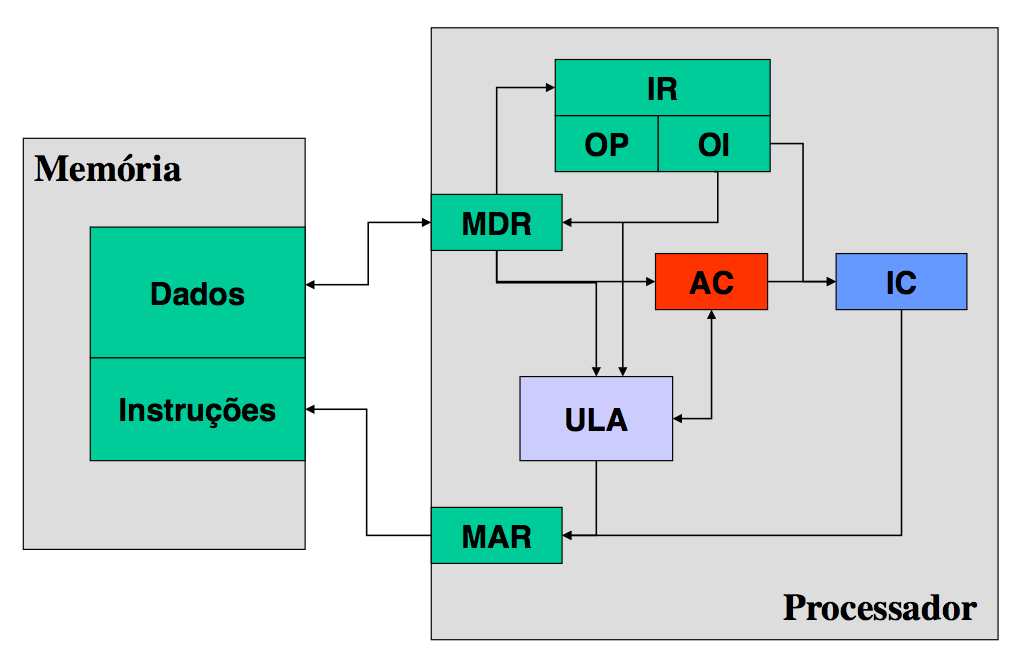
\includegraphics[width=\textwidth]{images/arquitetura-mvn.png}
	\label{fig:arquitetura-mvn}
\end{figure}

A arquitetura de Von Neumann é composta por um processador e uma memória principal. Na memória principal armazenam-se as instruções do código-fonte e os dados, sendo a divisão mostrada na figura~\ref{fig:arquitetura-mvn} apenas ilustrativa. Além da Unidade Lógica Aritmética (ULA), responsável pelo processamento de operações lógicas e aritméticas, o processador possui um conjunto de elementos físicos de armazenamento de informações e é comum dividir esses componentes nos seguintes módulos resgistradores:

\begin{enumerate}
	\item MAR - Registrador de endereço de memória
	
	Indica qual é a origem ou o destino, na memória principal, dos dados contidos no registrador de dados de memória.
	
	\item MDR -  Registrador de dados da memória
	
	Serve como ponte para os dados que trafegam entre a memória e os outros elementos da máquina.

	\item IC - Registrador de endereço de instrução 

	Indica a cada instante qual será a próxima instrução a ser executada pelo processador.

	\item IR -  Registrador de instrução

	Contém a instrução atual a ser executada. é subdividido em dois outros registradores, como na figura~\ref{fig:estrutura-ir}.
	\begin{figure}[ht]
		\centering
		\caption{Estrutura do registro de instrução (IR)}
		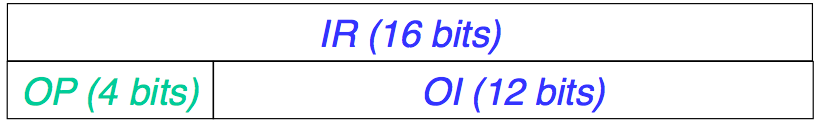
\includegraphics[width=0.8\textwidth]{images/estrutura-ir.png}
		\label{fig:estrutura-ir}
	\end{figure}

	\begin{enumerate}
		\item OP - Registrador de código de operação

		Parte do registrador de instrução que identifica a instrução que está sendo executada.

		\item OI - Registrador de operando de instrução

		Complementa a instrução indicando o dado ou o endereço sobre o qual ela deve agir.
	\end{enumerate}

	\item AC - Acumulador 

	Funciona como a área de trabalho para execução de operações lógicas ou aritméticas. Acumula o resultado de tais operações.
\end{enumerate}

A máquina executa um programa em diversos passos, listadas abaixo:

\begin{enumerate}
	\item Determinação da Próxima Instrução a Executar
	\item Fase de Obtenção da Instrução

	Obter na memória, no endereço contido no registrador de Endereço da Próxima Instrução, o código da instrução desejada.
	
	\item Fase de Decodificação da Instrução
	\label{item:decod-instrucao}

	Decompor a instrução em duas partes: o código da instrução e o seu operando, depositando essas partes nos registradores de instrução e de operando, respectivamente. Selecionar, com base no conteúdo do registrador de instrução, um procedimento de execução dentre os disponíveis no repertório do simulador (passo~\ref{item:exec-instrucao}).

	\item Fase de Execução da Instrução
	\label{item:exec-instrucao}
	
	Executar o procedimento selecionado no passo~\ref{item:decod-instrucao}, usando como operando o conteúdo do registrador de operando, preenchido anteriormente.
	
	Caso a instrução executada não seja de desvio, incrementar o registrador de endereço da próxima instrução a executar. Caso contrário, o procedimento de execução já terá atualizado convenientemente tal informação.
	
	\begin{enumerate}
		\item Execução da instrução (decodificada no passo~\ref{item:decod-instrucao})

		De acordo com o código da instrução a executar (contido no registrador de instrução), executar os procedimentos de simulação correspondentes (detalhados adiante).
		
		\item Acerto do registrador de Endereço da Próxima Instrução para apontar a próxima instrução a ser simulada:

		Incrementar o registrador de Endereço da Próxima Instrução.
	\end{enumerate}
	
\end{enumerate}
